\documentclass[colorthm]{./civarticle}
\usepackage{graphicx} % Required for inserting images
\usepackage[math]{blindtext}
\usepackage{float}


\title{esse 2}
\author{Захар Назаров}
\date{January 2024}

\begin{document}

\section{Введение}
В данной работе дается описание и некоторые аспекты безопасности следующих поточных шифров: DES и 3DES, AES, ГОСТ 34.12-2018 \textquotedblМагма\textquotedbl, ГОСТ 34.12-2018 \textquotedblКузнечик\textquotedbl, IDEA и IDEA NXT, RC6. Устройство шифра \textquotedblМагма\textquotedbl и его особенности рассматриваются более детально, также описаны атаки на него.

\section{Термины и определения}

\begin{definition}
  Сеть Фейстеля - это одна из архитектур блочного шифра. Исходный текст делится на блоки, и над каждым блоком производится одно и тоже преобразование. На вход этому преобразованию подается блок и ключ. Вот так выглядит это преобразование: 

  \begin{figure}[H]
      \centering
      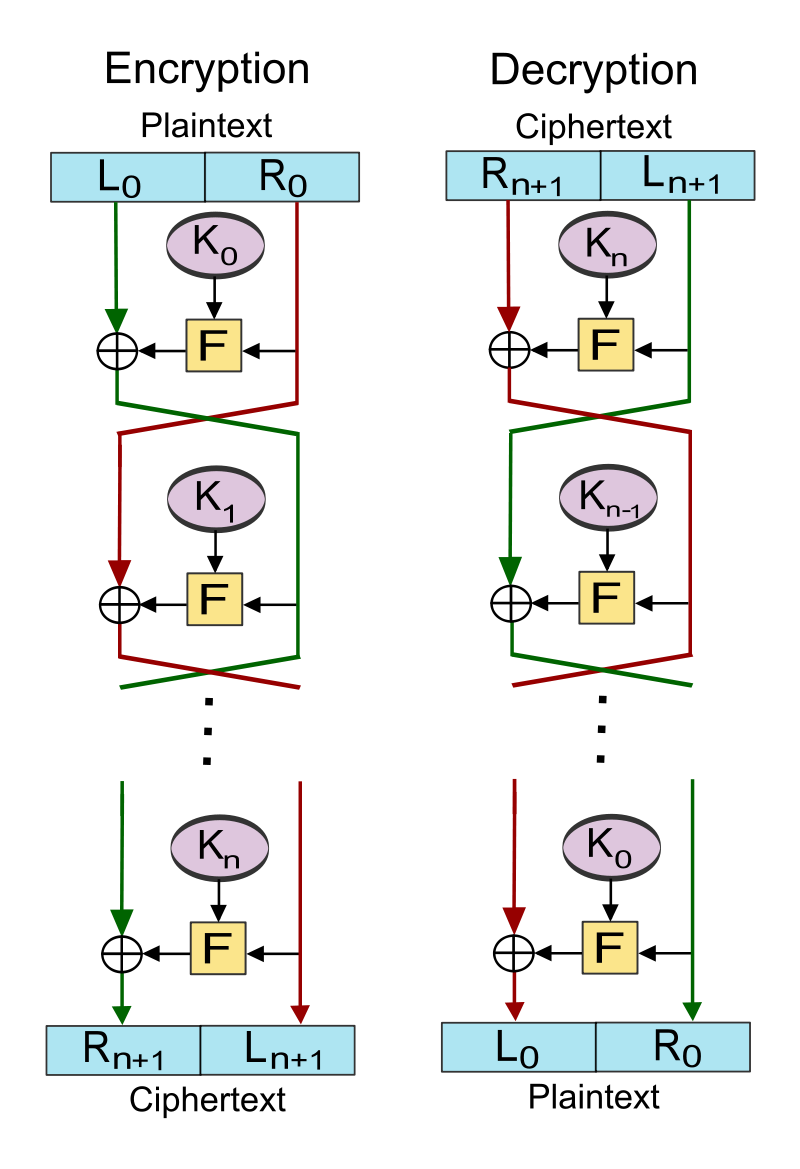
\includegraphics[width=0.5\linewidth]{800px-Feistel_cipher_diagram_en.svg.png}
      \caption{Сеть Фейстеля [17]}
      \label{fig:enter-label}
  \end{figure}

    Исходный текст (блок) делится на две части: $R_0, L_0$. Из ключа создаются подключи, количество которых ровно количеству раундов. После раунда ($L_i, R_i$) изменяется следующим образом:
    \begin{enumerate}
        \item $L_{i+1} = R_i$
        \item $R_{i+1} = L_i \oplus F(R_i, K_i)$
    \end{enumerate}

    Происходит N раундов, и $(L_n, R_N)$ является выходом преобразования. Причем последний раунд происходит без перестановки:

    \begin{enumerate}
        \item $L_{i+1} = L_i \oplus F(R_i, K_i)$
        \item $R_{i+1} = R_i$
    \end{enumerate}
    
    Функция $F$ может быть разной. Расшифрование происходит в обратном порядке.
  
\end{definition}

\begin{definition}
    S-блок (блок подстановоки, англ. S-box или substitution-box) - математическо преобразование, которое переводит n битов в m битов. n и m могут быть любыми. Обычно это преобразование представляется в виде таблицы.
\end{definition}

\begin{definition}
    P-блок (блок перестановки, англ. S-box или permutation-box) - математическое преобразование, которое перемешивает биты входной последовательности. По сути, это математическая перестановка.
\end{definition}

\begin{definition}
    SP-сеть (англ. Substitution–permutation network) - это композиция из идущих друг за другом S-блоков и P-блоков, которая используется в блочном шифровании. Обычно раундом блочного шифра, использующего классическую SP-сеть, называется преобразование блока данных с помощью одного S-блока, одного P-блока и ключа раунда.
\end{definition}

\begin{definition}
    Атака отражения (reflection attack) - это атака на сеть Фейстеля, которая использует сходство между функциями раунда, и с помощью их строит неподвижные точки полученной функции $f$: ${такие x: f(X) = x}$.
\end{definition}

\begin{definition}
    Атака \textquotedblчеловек посередине\textquotedbl (man-in-the-middle attack, MITM)- атака, предложеная Диффи Хеллманом [13], которая направлена на шифры со следующей конструкцией: $C = enc_{k_2}(enc_{k_1}(p))$. Основная идея атаки, это перебор ключей $k_1$, $k_2$ и поиск пар таких что: $enc^{-1}_{k_2}(C) = enc_{k_1}(P)$.
\end{definition}

\begin{definition}
    Сдвиговая атака (slide attack) - это атака на блочные шифры [14], на основе пар открытого текста и шифротекста, которая ищет такие пары $(C, P)$ и $C', P'$, что $F(P) = P', F(C) = C'$, где F - функция раунда. Далее ищется возможность восстановить весь секретный ключ или его часть из этой пары.
\end{definition}

\section{Шифры DES и 3DES}

\subsection{Шифр DES}
Шифр DES (Data Encryption Standard, стандарт шифрования данных) - это шифр, выбранный в качестве официального федерального стандарта обработки информации (FIPS) для США в 1976 году и впоследствии получивший широкое распространение на международном уровне.

\subsubsection{Описание шифра DES}

Блочный шифр DES принимает на вход 2 объекта: 64-битных блок данных и 64-битный секретный ключ. Схема шифра выглядит следующим образом: 

\begin{figure}[H]
    \centering
    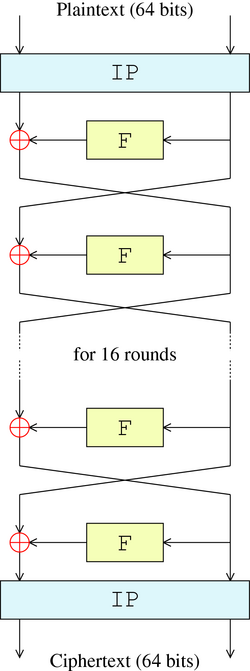
\includegraphics[width=0.25\linewidth]{DES-main-network.png}
    \caption{Устройство DES [1]}
    \label{fig:enter-label}
\end{figure}

Из схемы видно, что шифр состоит из блока инициализирующей перестановки, сети Фейстеля с 16 раундами и финальной перестановки. Рассмотрим функцию F из сети Фейстеля.

\textbf{Функция F сети Фейстеля}

F принимает на вход 32-битный блок данных и 48-битный ключ раунда. Схема фукнции выглядит следующим образом: 

\begin{figure}[H]
    \centering
    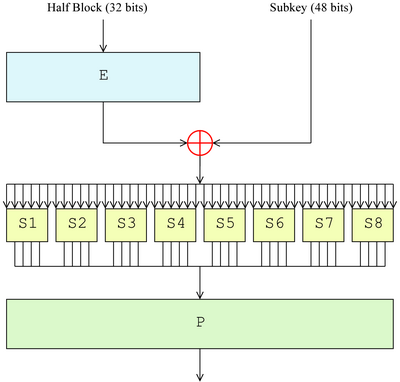
\includegraphics[width=0.5\linewidth]{DES-f-function.png}
    \caption{Функция F шифра DES [2]}
    \label{fig:enter-label}
\end{figure}

Сначала 32-битный блок данных преобразуется с помощью блока расширения E (cхема в Приложении этой работы) в 48-битный блок данных, который ксориться (xor) с 48-битным ключом раунда. Затем полученный блок делится на 8 6-битный частей, каждый из которых подается в соответствующий S-box $S_i$, который преобразует 6 битов в 4 бита. Далее 8 4-битных частей снова собираются в один 32-битный блок, который пропускается через блок перестановки P (cхема в Приложении этой работы), выходом которого является 32-битный блок. Полученный блок является выходом функции F.

\textbf{Вычисление ключей раунда}

В DES подается 64-битный секретный ключ, из которого далее для каждого раунда вычисляется ключа раунда. Схема этого вычисления выглядит следующим образом:

\begin{figure}
    \centering
    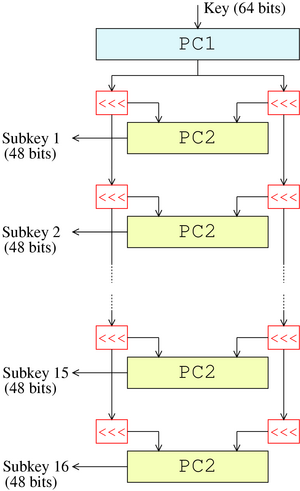
\includegraphics[width=0.5\linewidth]{DES-key-schedule.png}
    \caption{Расписание ключей шифра DES [3]}
    \label{fig:enter-label}
\end{figure}

Сначала 64-битный ключ подается в блок \textquotedblвыбора из перестановки 1\textquotedbl (Permuted Choice 1, PC1, cхема в Приложении этой работы), который выдает 56-битный блок данных. Этот блок делится на 2 28-битных блока $KL$ и $KR$. Затем каждый раунд ключ раунда $ROUNDKEY$ считается следующим образом:

\begin{enumerate}
    \item $KL = KL <<< 1$
    \item $KR = KR <<< 1$
    \item $ROUNDKEY = PC2(KL||KR)$
\end{enumerate}

Блок \textquotedblвыбора из перестановки 2\textquotedbl (Permuted Choice 2, PC2, cхема в Приложении этой работы), преобразует 56-битный блок данных, в 48-битный раунд ключа $ROUNDKEY$.

\subsubsection{Безопасность шифра}

Несмотря на большое количество работ с криптоанализом шифра DES, наилучшей атакой является метод грубой силы. Однако на сегодняшний день такая маленькая длина ключа делает его небезопасным. В 1998 году организация Electronic Frontier Foundation, используя специальный компьютер DES Cracker, вскрыла DES за 3 дня.

\subsubsection{Шифр 3DES}

Шифр 3DES был создан в 1978 году на основе алгоритма DES с целью устранения главного недостатка DES — малой длины ключа.

Входом шифра является 168-битный ключ $k$, который разбит на 3 равных ключа$(k_1, k_2, k_3)$. Шифрование 64-битного блока $P$ происходит следующим образом: 

\begin{equation}
    C = DES_{k_3}(DES^{-1}_{k_2}(DES_{k_1}(P)))
\end{equation}

$DES^{-1}$ это работа алгоритма DES в режиме расшифровки.

\textbf{Безопасность 3DES}

Достаточно старый 3DES остается невзломанным на сегодняшний день. По оценкам НИСТ этот шифр должен остаться надежным до 2030-х годов. Однако у него есть недостаток - это низкая скорость шифрования.

\section{Шифр AES}
2 января 1997 года NIST начинает искать преемника для DES, являвшегося американским стандартом с 1977 года. 2 октября 2000 года было объявлено, что победителем конкурса стал алгоритм Rijndael, и началась процедура стандартизации. AES (Advanced Encryption Standard) - стандарт шифрования в основе, которого лежит стандартизованный шифр Rijndael.

\subsubsection{Описание шифра AES}
Симметричный алгоритм блочного шифрования AES [4] -  SP-сеть с размером блока в 128 бит и ключом 128/192/256 бит.

Алгоритм оперирует матрицами 4x4, которые получены из 16-байтного (128-битного блока) набора $b_0, b_1, \dots, b_{15}$. Такая матрица в алгоритме называется состоянием (state):

\begin{equation}
    \left[\begin{array}{llll}
    b_0 & b_4 & b_8 & b_{12} \\
    b_1 & b_5 & b_9 & b_{13} \\
    b_2 & b_6 & b_{10} & b_{14} \\
    b_3 & b_7 & b_{11} & b_{15}
    \end{array}\right]
\end{equation}

Количество раундов зависит от длины ключа: 

\begin{itemize}
    \item[$\blacksquare$] 10 раундов для 128-битного ключа
    \item[$\blacksquare$] 12 раундов для 192-битного ключа
    \item[$\blacksquare$] 14 раундов для 256-битного ключа
\end{itemize}

Ознакомимся с базовыми функциями AES: SubBytes. ShiftRows,MixColumns,AddRoundKey.

\textbf{SubBytes}

На вход подается фукнции подается 1 байт (8 бит) из состояния. Многочленом $m(x) $AES в поле $GF(2^8)$ является: $m(x) = x^8+x^4+x^3+x+1$. Далее входное значение проходит 2 этапа:

\begin{enumerate}
    \item Находится обратный мультипликативный элемент к входному значению (8 битов интерпретируется как коэффициенты многочлена) в поле $GF(2^8)$ относительно $m(x)$.
    \item Пусть $x_0, x_1, \dots, x_7$ результат с прошлого шага. Далее происходит следующее преобразование: 

    \begin{equation}
        \left[\begin{array}{l}
y_0 \\
y_1 \\
y_2 \\
y_3 \\
y_4 \\
y_5 \\
y_6 \\
y_7
\end{array}\right]=\left[\begin{array}{llllllll}
1 & 0 & 0 & 0 & 1 & 1 & 1 & 1 \\
1 & 1 & 0 & 0 & 0 & 1 & 1 & 1 \\
1 & 1 & 1 & 0 & 0 & 0 & 1 & 1 \\
1 & 1 & 1 & 1 & 0 & 0 & 0 & 1 \\
1 & 1 & 1 & 1 & 1 & 0 & 0 & 0 \\
0 & 1 & 1 & 1 & 1 & 1 & 0 & 0 \\
0 & 0 & 1 & 1 & 1 & 1 & 1 & 0 \\
0 & 0 & 0 & 1 & 1 & 1 & 1 & 1
\end{array}\right]\left[\begin{array}{l}
x_0 \\
x_1 \\
x_2 \\
x_3 \\
x_4 \\
x_5 \\
x_6 \\
x_7
\end{array}\right]+\left[\begin{array}{l}
1 \\
1 \\
0 \\
0 \\
0 \\
1 \\
1 \\
0
\end{array}\right]
    \end{equation}
\end{enumerate}

Вектор $(y_0, y_1, \dots, y_7)$ является выходом функции SubBytes.

\textbf{ShiftRows}

На вход функции подается состояние (state). Первая строка состояния остается неизменной. Вторая, третья и четвертая строка сдвигаются циклически влево на 1 байт, 2 байта и 3 байта соотвественно. Выходом функции является полученное \textquotedblсдвинутое\textquotedbl состояние.

\textbf{MixColumns}

На вход функции подается состояние (state). Каждый столбец рассматривается как полином 4ой степени: $b_3*x^3+b_2*x^2+b_1$ в поле $GF(2^8)$. Каждый такой столбец умножается на фиксированный полином $a(x)$ по модулю $x^4+1$. $a(x) = 3*x^3+x^2+x+2$. Полученное новое состояние является выходом функции MixColumns. Также умножение полиномов можно представить в следующем виде:

\begin{equation}
    \left[\begin{array}{l}
d_0 \\
d_1 \\
d_2 \\
d_3
\end{array}\right]=\left[\begin{array}{llll}
2 & 3 & 1 & 1 \\
1 & 2 & 3 & 1 \\
1 & 1 & 2 & 3 \\
3 & 1 & 1 & 2
\end{array}\right]\left[\begin{array}{l}
b_0 \\
b_1 \\
b_2 \\
b_3
\end{array}\right]
\end{equation}

Все операции выполняются по модулю $2^8$.

\textbf{AddRoundKey}

На вход функции подается состояние (state) и ключ раунда. Выходом фукнции является сумма по модулю 2 состояния и ключа раунда.

\textbf{Вычисление ключей раунда}

На вход подается 128/192/256 битный ключ, который преобразуется в расширенный ключ длиной равной (количество раундов +1) * (длина блока). Для 128-битного ключа получится: (10 + 1) * 128 = 1408 бит. Далее каждый раунд от этого ключа берутся по 128 бит, которые и будут ключом раунда. Для первого ключа первые 128 бит расширенного ключа, для второго - вторые 128 бит и так далее. Для 128 и 192 битного ключа алгоритм следующий:

\begin{figure}[H]
    \centering
    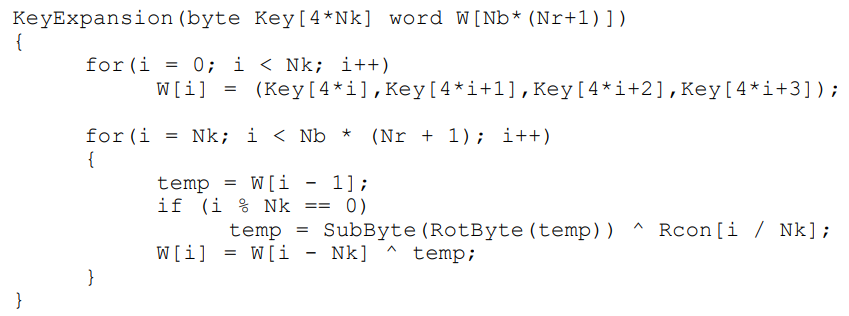
\includegraphics[width=0.5\linewidth]{key_shedule_1.png}
    \caption{Алгоритм вычисления расширенного ключа из секретного ключа длиной 128 или 192 бит}
    \label{fig:enter-label}
\end{figure}

Для 128 бит Nk = 4, для 192 бит Nk = 6. Для 128 бит Nr = 10, для 192 бит Nr = 12. Первые байты расширенного ключа равны секретному ключу.

Для 256 битного ключа алгоритм следующий:

\begin{figure}[H]
    \centering
    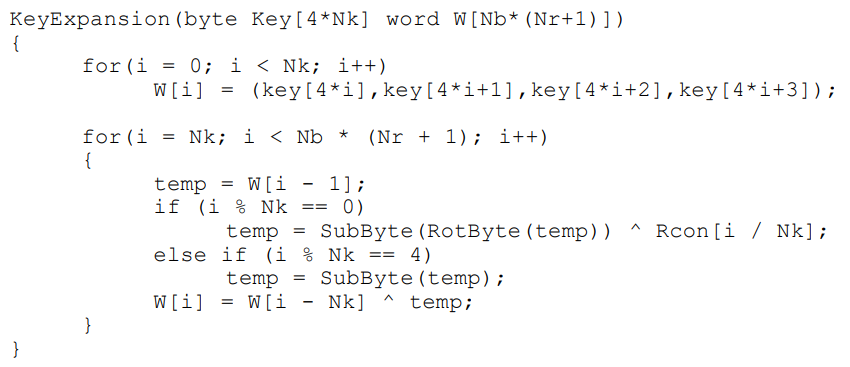
\includegraphics[width=0.5\linewidth]{key_shedule_2.png}
    \caption{Алгоритм вычисления расширенного ключа из секретного ключа длиной 256 бит}
    \label{fig:enter-label}
\end{figure}

Для 256 бит Nk = 8, Nr = 14.

Фукнция SubByte это старое название SubBytes. RotByte делает циклический сдвиг 4-байтного слова на один байт. Rcon (константа раунда) расчитывается так: $Rcon(i) = [rc(i), 00_{16}, 00_{16}, 00_{16}]$. Где $rc_i$  это 8-битное значение, которое считается так:

\begin{equation}
    rc_i= \begin{cases}1 & \text { if } i=1 \\ 2 \cdot r c_{i-1} & \text { if } i>1 \text { and } r c_{i-1}<80_{16} \\ \left(2 \cdot r c_{i-1}\right) \oplus 11 \mathrm{~B}_{16} & \text { if } i>1 \text { and } r c_{i-1} \geq 80_{16}\end{cases}
\end{equation}

\textbf{Основной алгоритм AES}

Теперь приведем основной алгоритм шифра AES [4]. На вход ему подается 128-битный блок данных (State) и 128/192/256-битный ключ (CipherKey). Функция раунда выглядит следующим образом:

\begin{figure}[H]
    \centering
    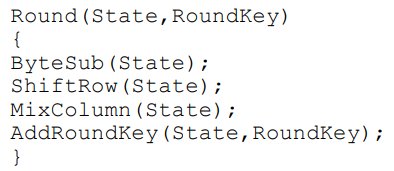
\includegraphics[width=0.25\linewidth]{round.png}
    \caption{Функция раунда алгоритма AES [4]}
    \label{fig:enter-label}
\end{figure}

Функция финального раунда отличается тем, что в ней нет функции MixColumns. Финальный раунд выглядит следующим образом:

\begin{figure}[H]
    \centering
    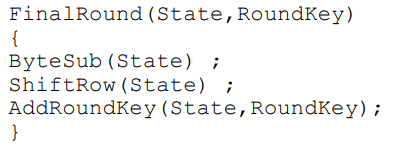
\includegraphics[width=0.25\linewidth]{f_round.png}
    \caption{Финальный раунд алгоритма AES [4]}
    \label{fig:enter-label}
\end{figure}

Основной алгоритм шифра AES выглядит следующим образом:

\begin{figure}[H]
    \centering
    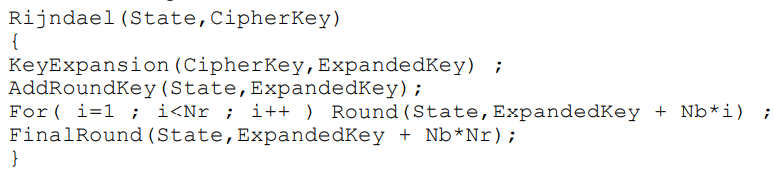
\includegraphics[width=0.5\linewidth]{aes.png}
    \caption{Шифр AES [4]}
    \label{fig:enter-label}
\end{figure}

\subsubsection{Безопасность шифра}
На сегодняшний день не было опубликовано реальных атак на шифр AES. В 2003 году агенство национальной безопасности США постановило, что шифр AES является достаточно надежным, чтобы использовать его для защиты сведений, составляющих государственную тайну [6].


\section{Шифр ГОСТ 34.12-2018 \textquotedblМагма\textquotedbl}

В марте 1978 года после предварительного изучения опубликованного в 1976 году стандарта DES началась разработка алгоритма шифрования в рамках темы «Магма» (защита информации криптографическими методами в ЭВМ ряда Единой Системы). Позже алгоритм был утверждён постановлением Госстандарта СССР № 1409 от 2 июня 1989 года.

\subsubsection{Описание шифра \textquotedblМагма\textquotedbl}
 
Шифр \textquotedblМагма\textquotedbl - это сеть Фейстеля с 32 раундами, которая принимает на вход 64-битный блок данных. Длина секретного ключа - 256 бит, длина ключа раунда - 32 бита.

\textbf{Функция F сети Фейстеля}

Преобразование $F$ в Магме выглядит следующим образом:

\begin{figure}[H]
    \centering
    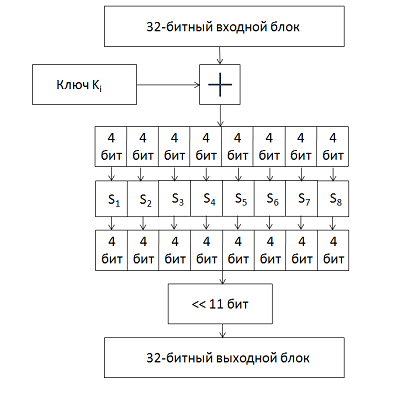
\includegraphics[width=0.25\linewidth]{Feistel_function_GOST.png}
    \caption{Функция F в Магме [7]}
    \label{fig:enter-label}
\end{figure}

В $F$ поступают 32-битный блок и 32-битный ключ раунда. Сначала они перемешиваются с помощью побитового сложения по модулю 2, затем полученный блок бьется на 8 разных частей и к каждой части применяется свой S-box. Выходы S-box'ов обратно собираются в один блок, который сдвигается циклически влево на 11 бит и далее подается на выход $F$.

\textbf{Вычисление ключей раунда}

На вход подается 256-битный секретный ключ $K=k_0||\dots||k_{256}$. Ключ раунда i вычисляется по следующей формуле:

\begin{equation}
    \begin{split}
        k_{8-i} = k_{32*(i+1)-1}||\dots||k_{32*i}, i=0,1,\dots,7 \\
    k_{i+8} = k_i, i=1,2,\dots,8 \\
    k_{i+16} = k_i, i=1,2,\dots,8 \\
    k_{i+24} = k_{9-i}, i=1,2,\dots,8  
    \end{split}
\end{equation}

\subsubsection{Эксплуатационные и технические характеристики}

В стандарте [8] изначально предусмотрели несколько режимов его работы. Выше описан шифр Магма, работающий в режиме простой замены. 

\textbf{Режим гаммирования}

Блочный шифр Магма может работать как поточный шифр, создавая ключевую последовательность. Для этого необходимо задать синхропосылку 64-битную синхропосылку S, которая будет открыто передаваться вместе с шифротекстом. Алгоритм работы шифра в режиме гаммирования выглядит следующим образом:

\begin{enumerate}
    \item Синхропосылка S заносится в регистры $N_1$ и $N_2$ шифруется с помощью Магмы в режиме простой замены с секретным ключом K. Полученное значение переписывается в вспомогательные 32-битные регистры $N_3$ и $N_4$.
    \item $N_3 = N_3 + C_2 mod 2^{32}$, где $C_2 = 1010101_{16}$.
    \item $N_4 = N_4 + C_1 mod (2^{32} - 1)$, где $C_1 = 1010104_{16}$.
    \item Затем $N_3$ и $N_4$ в рабочие регистры шифра $N_1$ и $N_2$ (левая и правая часть 64-битного блока данных) соотвественно. Этот блок шифруется с помощью шифра в режиме простой замены. Полученный блок является первой 64-битной гаммой.
    \item Следующие гаммы высчитываются шагами 2-4  в соответствии с длиной шифруемого текста.
\end{enumerate}

Особенностью этого режима является то, что если поменять один бит зашифрованного текста, то поменяется одни расшифврованного текста. При обычном режиме такого эффекта нет.

\textbf{Режим гаммирования с обратной связью}

Этот режим похож на предыдущий. Основное отличие в том, что он подмешивает в текущую гамму шифротекст с предыдущего шага. Пусть у нас есть синхропосылка S. Алгоритм выглядит так: 

\begin{enumerate}
    \item Синхропосылка S заносится в регистры $N_1$ и $N_2$
    \item Содержимое регистров $N_1$ и $N_2$ шифруется в режиме простой замены. Полученный блок является гаммой.
    \item $N_4 = N_4 + C_1 mod (2^{32} - 1)$, где $C_1 = 1010104_{16}$.
    \item Гамма подмешивается в блок открытого текста. Полученный блок идет на выход как шифротекст, и также заносится в регистры $N_1$ и $N_2$ для расчета следующей гаммы.
    \item Следующие гаммы высчитываются шагами 2-3 в соответствии с длиной шифруемого текста.
\end{enumerate}

\textbf{Режим выработки имитовставки}
Это особый режим работы, который считает преобразует шифротекст в последовательность длины L бит ($1 <= L < 32)$. Этот \textquotedblслепок\textquotedbl открытого текста может отправляться вместе с шифротекстом, полученным в одном из режимов, описанных выше, для того, чтобы проверять целостность пришедших данных. Так выглядит схема работы шифра в этом режиме:

\begin{figure}[H]
    \centering
    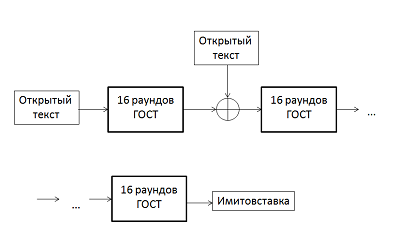
\includegraphics[width=0.25\linewidth]{Imitovstavka_GOST.png}
    \caption{Режим выработки имитовставки [6]}
    \label{fig:enter-label}
\end{figure}

\textquotedblСлепок\textquotedbl вырабатывается для более чем 1 блоков открытого текста по 64 бит. Алгоритм следующий:

\begin{enumerate}
    \item Блок данных загружается в $N_1$ и $N_2$. После чего шифруется режиме простой замены только первые 16 раундов.
    \item К полученному результату подмешивается (побитовая сумма по модулю 2) следующий блок открытых данных. Для последнего блока ничего не подмешивается.
\end{enumerate}

От полученного блока берется последовательность с $32-L$ бита по $32$ (нумерация с 1). Стандарт рекомендует выбирать L так, что вероятность навязывания ложных данных равна $2^{-L}$.

Выработка имитовставки может производится параллельно вычислению шифротекста. Но отправляется она в самом конце.

\textbf{Возможности реализации и скорость работы}

Магму можно реализовать как аппаратно, так и программно. В программной реализации ГОСТ как любой шифр сети Фейстеля медленнее современных шифров типа AES (SP-сети). Однако реализация ГОСТа явно быстрее чем его конкурент 3DES. 

Если сравнивать аппаратные реализации, то для ГОСТа требутеся существенно меньше элементов для его построения, чем для того же AES[9]. В работе [10] смогли за 651 GE(gate Equivalent) построить Магму против 3000 GE для AES!Поэтому он является лидером в нише недорогих и безопасных решений. 

Однако при должном количестве ресурсов реализациия SP-сети быстрее чем сеть Фейстеля, так как SP-сеть изначально подается лучшей параллелизации. 

В работе [11] скорость программной реализации Магмы в среднем была 135 МБ/с. 

\subsection{Атаки}

Более 20 лет с момента создания шифра (до 2011 года) шифр Магма считался очень надежным, несмотря на многочисленные попытки его взломать.

\subsubsection{Слабые ключи}

В работе [16] было показано что существуют слабые ключи для шифра Магма.

\textbf{Угроза и модель нарушителя} 

Данная атака направлена на поиск слабых ключей из пар открытого текста и шифротекста, поэтому это атака на основе знания открытого текста (known-plaintext attack, KPA).

\textbf{Описание атаки} 

Общий вид секретного ключа выглядит так: $K = K_1||K_2||K_3||K_4||K_5||K_6||K_7||K_8$. Слабые ключи имеет структуру:

\begin{enumerate}
    \item $K$ - палиндром. Порождает 8-подобный шифр.
    \item $K = (A||B||C||D||D||B||C||A)$. Порождает 4-подобный шифр.
    \item $K = (A||А||A||А||A||А||A||А)$. Порождает 1-подобный шифр.
\end{enumerate}

Такие ключи уменьшают пространство перебора для таких ключей, также позволяют провести сдвиговую атаку с дополнением (сomplementation slide).

\textbf{\emph{Оценка требуемых ресурсов для атаки}}

При атаке полным перебором размерность ключевого пространства уменьшается до $2^{128}, 2^{32}$ при этом шанс на такой ключ пренебрежима мала.

\textbf{\emph{Возможности практической реализации атаки}}

Эта атака непрактична так, как очень низкая вероятность успеха. Однако она предворяет другие атаки.

\textbf{\emph{Пути нейтрализации атаки}}. В данной атаке используется простота расписания ключей. Усложнив алгоритм вычисления ключей раунда, можно помешать данной атаке.

\subsubsection{Сдвиговая атака}

В 2000 году была предложена сдвиговая атака [15] на последние 20 раундов шифра Магма, в котором ключ в функции F складывается по модулю два с 32-битным блоком.

\textbf{Угроза и модель нарушителя} 

Данная атака направлена на восстановление последних 128 битов секретного ключа из пар открытого текста и шифротекста, поэтому это атака на основе знания открытого текста (known-plaintext attack, KPA).

\textbf{Описание атаки}.

Применяется сдвиг с поворотом (Sliding with a twist) [14] для следующей цепочки блоков:

\begin{equation}
    \begin{aligned}
& \begin{array}{llllllllllllllllllllllll}
K_4 & K_5 & K_6 & K_7 & K_0 & K_1 & K_2 & K_3 & K_4 & K_5 & K_6 & K_7 & K_7 & K_6 & K_5 & K_4 & K_3 & K_2 & K_1 & K_{0^{\bullet}}
\end{array} \\
& \begin{array}{llllllllllllllllllll}
K_0 & K_1 & K_2 & K_3 & K_4 & K_5 & K_6 & K_7 & K_7 & K_6 & K_5 & K_4 & K_3 & K_2 & K_1 & K_0 & K_7 & K_6 & K_5 & K_4
\end{array} \\
&
\end{aligned}
\end{equation}

Обозначим за F 4 раунда шифра с ключами $K_4, \dots, K_7$. В $2^{64/2}=2^{33}$ парах открытого текста и шифротекста ожидаемо найдутся 2 парs сдвига для функции F (парадокс дня рождении). Если пара найдена, то подбор ключа $K_4, \dots, K_7$ займет около $2^{9}$ запусков 4-раундовой версии шифра (или $2^5$ 20 раундовых версии). Изучив все пары, которых $\frac{2^{33}*(2^{33}-1)}{2} \approx 2^{65}$, мы найдем для каждой своего кандидата на 128-битный ключ и сохраним в таблицу. Правильный ключ должен появится дважды.

Далее нетрудно найти $K_0, \dots, K_3$. Мы можем отделить первые 4 раунда и в том же пуле текстов искать неподвижные точки, так как последние 16 раундов образуют палиндром (первые 8 ключей в прямом порядке, последние 8 ключей в инвертированном). Всего $2^{32}$ значений явлвяются неподвижными точками. Из них выбирается 2 кандидата, и затем по первым 4 раундам с $K_0, \dots, K_3$ этот же ключ и восстанавливается за те же $2^5$ операции. Полученный 256-битный ключ проверяется на какой-нибудь паре.

\textbf{\emph{Оценка требуемых ресурсов для атаки}}

Это атака требует $2^{33}$ пар открытого текста и шифротекста, $2^{65}$ блоков памяти, а также $2^{70}$ операции шифрования.

\textbf{\emph{Возможности практической реализации атаки}}

Большое количество затрат по памяти делают эту атаку непрактичной.

\textbf{\emph{Пути нейтрализации атаки}}. В данной атаке используется простота расписания ключей. Усложнив алгоритм вычисления ключей раунда, можно помешать данной атаке.


\subsubsection{Атака Reflection-Meet-in-the-Middle Attack}
В феврале 2011 года на конференции FSE была представлена атака нового типа Reflection-Meet-in-the-Middle Attack [12] на шифр ГОСТ. Это атака требует $2^{32}$ пар открытого текста и шифротекста, $2^{64}$ блоков памяти, а также $2^{225}$ операции шифрования. Заметим, что уже намного лучше атаки полного перебора, требующей $2^{256}$ операции шифрования.

\textbf{Угроза и модель нарушителя} 

Данная атака направлена на восстановление секретного ключа из пар открытого текста и шифротекста, поэтому это атака на основе знания открытого текста (known-plaintext attack, KPA).

\textbf{Описание атаки}

Это атака отталкивается от расписания ключей, которое можно представить схемой:

\begin{figure}
    \centering
    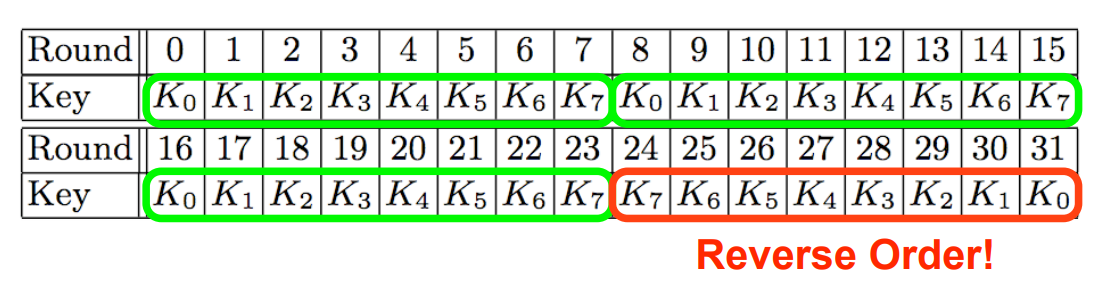
\includegraphics[width=0.5\linewidth]{Снимок экрана 2024-01-17 162824.png}
    \caption{Вычисление ключей раунда шифра Магма [10]}
    \label{fig:enter-label}
\end{figure}

Это значит, что схему шифрования для секретного ключа K можно записать так:

\begin{equation}
    \begin{aligned}
E_K & =S \circ F_K[25,32] \circ F_K[17,24] \circ F_K[9,16] \circ F_K[1,8] \\
& =F_K^{-1}[1,8] \circ S \circ F_K[1,8] \circ F_K[1,8] \circ F_K[1,8] .
\end{aligned}
\end{equation}

Где $F[i, j]_k$ - это функция F схемы Фейстеля, а $S$ - перестановка двух 32-битных слов 64-битного блока. В атаке отражения утверждается, что существует $2^{32}$ входных блоков $x$, таких что $F_K^{-1}[1,8] \circ S \circ F_K[1,8](x) = x$. То есть вероятность, что случайный блок будет таким равна: $P_{ref}=\frac{2^{32}}{2^{64}}=2^{-32}$. Таким образом, для этих неподвижных точек существенными является только первые 16 раундов. Такая точка точно есть в $2^{32} + 1$ случайных блоках. Поэтому считаем, что у нас найдена такая точка, осталось разобраться с первыми 16 раундами.

Из-за того, что в первых 16 раунда ключами раунда по сути являются 2 подряд идущих секретных ключа, поделенные на блоки, то можно записать схему шифрования так:

\begin{equation}
    E_K & = F_K[1, 8] \circ F_K[1,8] \\
    & = F_K[5, 8] \circ F_K[1,4] \circ F_K[5, 8] \circ F_K[1,4]
\end{equation}

\begin{definition}
    Множество $Z$ эквивалентных ключей на $F_k[i, j]$ для пары $x, y \in {0, 1}^{64}$ это:
    \begin{equation}
        Z(F_k[i, j], x, y) = {ek \in {0, 1}^{256} : F_{ek}[i, j](x) = y}
    \end{equation}
\end{definition}

У шифра Магма есть следующее свойство:

\begin{remark}
    Для заданных $x, y$ легко найти $Z(F_k[1, 4], x, y)$ и $Z(F_k^{-1}[5, 8], x, y)$, мощность каждого множества равна $2^{64}$.
\end{remark}

Доказательство приводится в [12]. Коротко идея заключается в том, что если мы выберем $x, y$ и первые два ключа раунда $k_1, k_2$, то мы легко можем однозначно получить ключи $k_3, k_4$, такие что $k_1||k_2||k_3||k_4 \in Z(F_k[1, 4], x, y)$ (причем мы получим все ключи Z). Аналогично для $Z(F_k^{-1}[5, 8], x, y)$ будут найдены все $k_5||k_6||k_7||k_8$. Мы смогли разбить секретный ключ $k = k_1||k_2||k_3||k_4||k_5||k_6||k_7||k_8$ на все левые его части $K_a$ и все правые части $K_b$ на два независимых подмножества $Z_{K_a}(F_k[1, 4], x, y)$, $Z_{K_b}(F_k^{-1}[5, 8], x, y)$.

Нам дана пара открытого текста $P$ и шифротекста $C$. Пусть $S = F_K[1, 4](P)$ и $T = F^{-1}_K[5, 8](C)$. Для них мы можем легко найти $Z_{K_a}(F_k[1, 4], P, S)$, $Z_{K_b}(F_k^{-1}[5, 8], C, T)$. Теперь мы можем провести MITM атаку, игнорируя первые 4 раунда и последние 4 раунда, между $F^{-1}_K[5, 8](S)$ и $F^_K[1, 4](T)$. Cхема атаки выглядит следующим образом: 

\begin{figure}
    \centering
    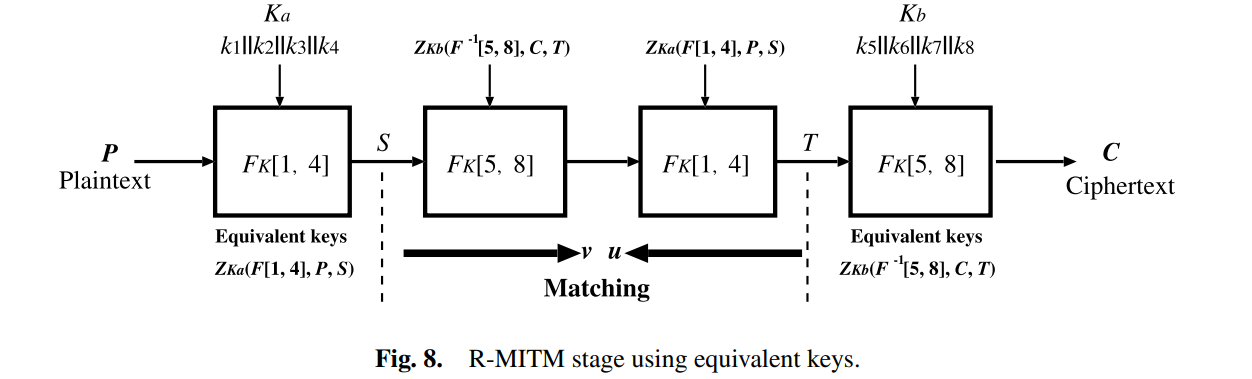
\includegraphics[width=0.75\linewidth]{mitm.png}
    \caption{R-MITM атака на Магму [12]}
    \label{fig:enter-label}
\end{figure}

Пусть дана пара открытого текста и шифротекста $P$ и $C$. Алгоритм атаки следующий:

\begin{enumerate}
    \item Выбираем произвольные $S$ и $T$.
    \item Cчитаем множества $Z_{K_a}(F_k[1, 4], P, S)$, $Z_{K_b}(F_k^{-1}[5, 8], C, T)$.
    \item Для каждого ключа $K_b$ из $Z_{K_b}(F_k^{-1}[5, 8], C, T)$ считаем $v = F_{K_b[5,8](S)}$ и запоминаем в таблицу $(v, K_b)$.
    \item Для каждого ключа $K_a$ из $Z_{K_a}(F_k[1, 4], P, S)$ считаем $u = F_{K^{-1}_a[1,4](T)}$.
    \item Если $u=v$, то запоминаем ключ $K=K_a||K_b$ как кандидата на истинный ключ. Число таких ключей будет $2^{64}$.
    \item Повторяем шаги $2-5$ для всевозмонжных $S$ и $T$ ($2^{128} раз$).
\end{enumerate}

После этого останется $2^{128} * 2^{64} = 2^{192}$ ключей-кандидатов. К этому моменту мы отсеяли ключи, которые точно не могут быть истиным ключом, поэтому в этом списке точно будет истиный ключ. Дальше он ищется в этом списке полным перебором по другим известным парам открытого текста и шифротекста.

$Z_{K_a}(F_k[1, 4], P, S)$ содержит $2^{64}$ ключей различных ключей. Причем для разных $P$ также разные множества ключей, так как атака предполагает что S-box'ы биективны. Количество $P$ также равно $2^{64}$, поэтому в алгоритме мы переберем всевозмножные левые части $K_a$ секретного ключа: $2^{64}*2^{64}$. Также для $K_b$, поэтому будут учетные всевозможные ключи.

Осталось не забыть, что этот алгоритм делается для каждой пары $P$ и $С$ из известных нам пар, которых $2^{64}$. Таким образом сложность атаки равна:

\begin{equation}
    \begin{aligned}
C_{\text {comp }} & =(\underbrace{\left(2^{128}\left(2^{64}+2^{64}\right)\right)}_{\text {R-MITM stage }}+\underbrace{\left(2^{256-64}+2^{256-128}+\cdots\right)}_{\text {Key testing stage }}) \times 2^{32}=2^{225} .
\end{aligned}
\end{equation}

\textbf{\emph{Оценка требуемых ресурсов для атаки}}

Это атака требует $2^{32}$ пар открытого текста и шифротекста, $2^{64}$ блоков памяти, а также $2^{225}$ операции шифрования.

\textbf{\emph{Возможности практической реализации атаки}}

Такое количество операции на сегодняшний день невозможно выполнить за обозримое время, также нельзя собрать такое количество пар открытого текста и шифротекста в реальной жизни. Эта атака имеет теоритическую ценность, а не практическую.

\textbf{\emph{Пути нейтрализации атаки}}. В данной атаке используется простота расписания ключей. Усложнив алгоритм вычисления ключей раунда, можно помешать данной атаке.

\subsection{Заключение}
Шифр Магма довольно долго и усердно разрабывался. Полученная схема шифрования очень компактно реализуется на аппаратном уровне, при это обеспечивая высокую скорость. Более 20 лет специалисты не могли подступиться к данному шифру, но уже начали появляться атаки более быстрые чем полный перебор. Основным его недостатком является это довольно простое расписание ключей. При этом атаки требуют достаточно специфичных условий. Это может быть нецелесообразно в случаях, когда шифр использутся как недорогой и быстрый вариант.

\section{Шифр ГОСТ 34.12-2018 \textquotedblКузнечик\textquotedbl}

Шифр \textquotedblКузнечик\textquotedbl был впервые утверждён  в качестве стандарта в ГОСТ Р 34.12-2015 «Информационная технология. Криптографическая защита информации. Блочные шифры». В 2018 году он получил международную стандартизацию [17]. 

\subsubsection{Описание шифра \textquotedblКузнечик\textquotedbl}

\textquotedblКузнечик\textquotedbl - симметричный алгоритм блочного шифрования с 128-битным блоком и 256-битным ключом, основанный на SP-сети с 10 раундами.

Для описания шифра потребуется ввести следующие обозначения:

\begin{enumerate}
    \item $F$ - конечное поле $GF(2)[x]/p(x)$, где $p(x) = x^8+x^7+x^6+x+1$. Элементы поля представляются целыми числами: коэффициенты при степенях двойки это коэффициенты многочлена.
    \item $\delta: V_8 -> F$ ставит в соотвествие двоичной строке элемент из $F$, $\delta^{-1}$ - отображение, обратное к $\delta$. 
    \item $N(a) = S(a_{15})||\dots||S(a_{0})$
    \item $S$ - нелинейное преобразование заданное в виде конкретной подстановки (cхема в Приложении этой работы).
    \item $G(a) = \gamma(a_{15}, \dots, a_0)||a_15||\dots||a_1$.
    \item $H(a) = G^{16}(a)$.
    \item $Add_2[k](a) k \oplus a$.
    
\end{enumerate}

\begin{equation}
    \begin{aligned}
& \gamma\left(a_{15}, \ldots, a_0\right)=\delta^{-1}\left(148 * \delta\left(a_{15}\right)+32 * \delta\left(a_{14}\right)+133 * \delta\left(a_{13}\right)+16 * \delta\left(a_{12}\right)+\right. \\
& 194 * \delta\left(a_{11}\right)+192 * \delta\left(a_{10}\right)+1 * \delta\left(a_9\right)+251 * \delta\left(a_8\right)+1 * \delta\left(a_7\right)+192 * \delta\left(a_6\right)+ \\
& \left.194 * \delta\left(a_5\right)+16 * \delta\left(a_4\right)+133 * \delta\left(a_3\right)+32 * \delta\left(a_2\right)+148 * \delta\left(a_1\right)+1 * \delta\left(a_0\right)\right),
\end{aligned}
\end{equation}

\textbf{Шифр \textquotedblКузнечик\textquotedbl}

\begin{equation}
    Enc(a) = Add_2[K_10]HNAdd_2[K_9]\dots HNAdd_2[K_2]HNAdd_2[K_1](а), a это 128-битный блок.
\end{equation}

Расшифрование происходит в обратном порядке и с обратными фукнциями. 

\textbf{Вычисление ключей раунда}

На вход подается 256-битный ключ $K = k_{256}||\dots||k_0$. Генерируются итерационные контсанты $C_i=H(Bin_{128}(i))$, $i = 1, 2, \dots, 32$. $Bin_{128}$ превращает число в его 128-битное двоичное представление. Далее ключи считаются так:

\begin{enumerate}
    \item $K_1 = K_{255}||\dots||K_{128}$
    \item $K_2 = K_{127}||\dots||K_{0}$
    \item $(K_{2i+1}, K_{2i+2} = F[C_{8(i-1)+8}]\dotsF[C_{8(i-1)+1}](K_{2i-1}, K_{2i})$, $i=1,2,3,4$.
\end{enumerate}

\subsubsection{Безопасность шифра}

В [18] было показано, что нелинейный этап алгоритма можно декомпозировать. Также есть MITM атака [19] на \textquotedblКузнечик\textquotedbl, требующая $2^{140}$ операции, $2^{153}$ памяти и $2^{113}$ данных.

\section{Шифры IDEA и IDEA NXT}

\subsection{Шифр IDEA}
В 1991 году компанией Ascom был создан шифр IDEA(International Data Encryption Algorithm).

\subsubsection{Описание шифра IDEA}

Шифр IDEA - это симметричный блочный шифр, который является модификацией сети Фейстеля с размером блока в 64 бит, 128-битным ключом и 8.5 раундами. Схема шифрование выглядит следующим образом:

\begin{figure}[H]
    \centering
    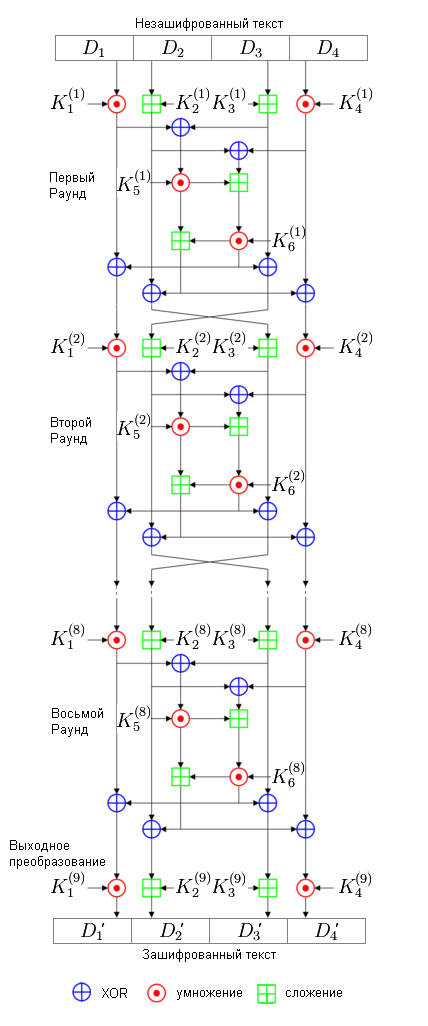
\includegraphics[width=0.5\linewidth]{IDEA_encryption.png}
    \caption{Шифр IDEA [20]}
    \label{fig:enter-label}
\end{figure}

\begin{figure}[H]
    \centering
    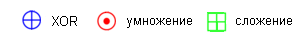
\includegraphics[width=0.5\linewidth]{Operations.png}
    \caption{Операции из схемы шифра IDEA [20]}
    \label{fig:enter-label}
\end{figure}

Таким образом, исходный 64-битнный блок делится на 4 равные части $D_1, D_2, D_3, D_4$ и проходит через 8.5 раундов, перемешиваясь с ключами раунда при помощи операции. После 8 одинаковых раундов происходит отдельный финальный раунд, который показан на схеме. Матиматически описание для первых 8 раундов ($i=1,\dots,8$) выглядит так:

\begin{equation}
    \begin{aligned}
& A^{(i)}=D_1^{(i-1)} * K_1^{(i)} \\
& B^{(i)}=D_2^{(i-1)}+K_2^{(i)} \\
& C^{(i)}=D_3^{(i-1)}+K_3^{(i)} \\
& D^{(i)}=D_4^{(i-1)} * K_4^{(i)} \\
& E^{(i)}=A^{(i)} \oplus C^{(i)} \\
& F^{(i)}=B^{(i)} \oplus D^{(i)} \\
& D_1^{(i)}=A^{(i)} \oplus\left(\left(F^{(i)}+E^{(i)} * K_5^{(i)}\right) * K_6^{(i)}\right) \\
& D_2^{(i)}=C^{(i)} \oplus\left(\left(F^{(i)}+E^{(i)} * K_5^{(i)}\right) * K_6^{(i)}\right) \\
& D_3^{(i)}=B^{(i)} \oplus\left(E^{(i)} * K_5^{(i)}+\left(F^{(i)}+E^{(i)} * K_5^{(i)}\right) * K_6^{(i)}\right) \\
& D_4^{(i)}=D^{(i)} \oplus\left(E^{(i)} * K_5^{(i)}+\left(F^{(i)}+E^{(i)} * K_5^{(i)}\right) * K_6^{(i)}\right)
\end{aligned}
\end{equation}

Для последнего раунда:

\begin{equation}
    \begin{aligned}
& D_1^{(9)}=D_1^{(8)} * K_1^{(9)} \\
& D_2^{(9)}=D_3^{(8)}+K_2^{(9)} \\
& D_3^{(9)}=D_2^{(8)}+K_3^{(9)} \\
& D_4^{(9)}=D_4^{(8)} * K_4^{(9)}
\end{aligned}
\end{equation}

\textbf{Вычисление ключей раунда}

На вход поступает 128-битный ключ, из которого для каждого из 8 раундов генерируется по 6 16-битных ключей, для финального раунда 4.

Сначала 128-битный ключ разбивается на 8 16-битных блоков: $K^(1)_1, K^(1)_2, K^(1)_3, K^(1)_4, K^(1)_5, K^(1)_6, K^(2)_1, K^(2)_2$. Затем этот ключ циклически сдвигается влево на 25 битов. После чего получаем следующие 8 16-битных ключей. Затем снова сдвигаем ключи, делаем это до тех пор пока не получим все 52 ключей раунда.

\subsubsection{Безопасность шифра}
У алгоритма существует большие классы слабых ключей. Есть примеры взлома IDEA c количеством раундов равным 6 [21].

\subsection{Шифр IDEA NXT}
В 2003 году институт EFPL представил преемника шифра IDEA - IDEA NXT, который также использует схему Лая-Месси (Lai–Massey scheme).

\subsubsection{Описание шифра IDEA NXT}
Шифр IDEA NXT [22] - это симметричный блочный шифр, который является модификацией сети Фейстеля с размером блока в 64/128 бит, [0-128]-битным ключом и 16 раундами. Схема шифрование выглядит следующим образом. Опишем 64-битную версию, ее раунд выгядит так:

\begin{figure}[H]
    \centering
    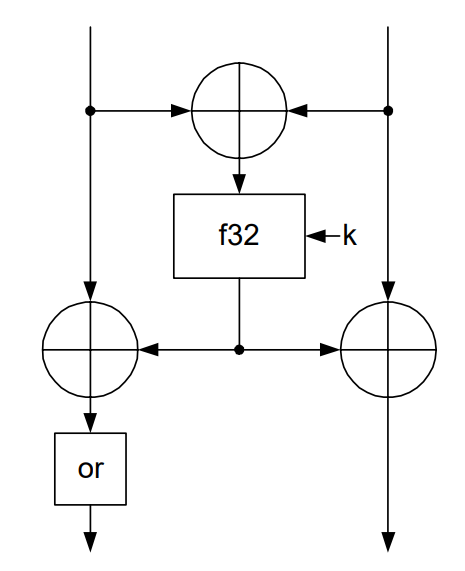
\includegraphics[width=0.25\linewidth]{64_rounds.png}
    \caption{Схема раунда IDEA NXT64 [22]}
    \label{fig:enter-label}
\end{figure}

Функция f32 принимает на вход 32-битный блок. Схема функции f32 выглядит следуюзим образом:

\begin{figure}[H]
    \centering
    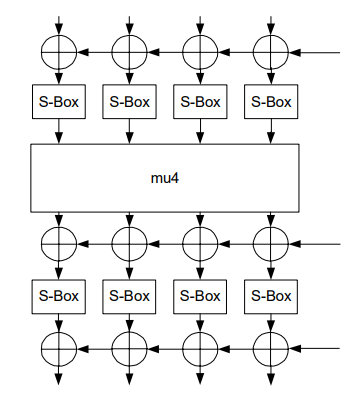
\includegraphics[width=0.25\linewidth]{f32.png}
    \caption{Функция f32 [22]}
    \label{fig:enter-label}
\end{figure}

Cледовательно f32 состоит из блока подстановки, блока подстановки и блока добавление ключа раунда.

\textbf{Вычисление ключей раунда}
Алгоритм на вход получает [0-256]-битный ключ с кратностью 8. В зависимости от длины ключа применяется конкретный алгоритм. Однако у всех общая схема: 

\begin{figure}[H]
    \centering
    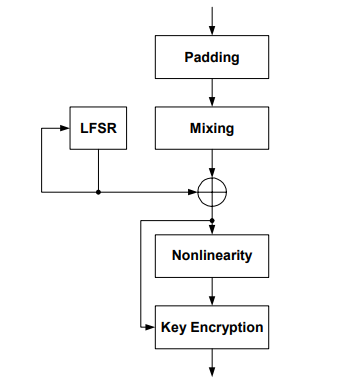
\includegraphics[width=0.25\linewidth]{foto.png}
    \caption{Схема вычисления ключей раунда [22]}
    \label{fig:enter-label}
\end{figure}

Сначала ключ расширяется до длины своей категории. Затем перемешивается с помощью рекурсии Фиббоначи. Затем идет диверсификационная часть, которая реализована с помощью LSFR и функции нелинейности. Конкретная реализация в документе [22] не приведена.

\subsubsection{Безопасность шифра}
В работе [23] описана атака на 64-битную версию. Он смогли атаковать 5/6/7 раундов с количеством требуемых операции $2^{71}, 2^{135}, 2^{199}$.


\section{Шифр RC6}
Шифр RC6 был создан и подан в 1998 году в NIST как один из кандидатов на роль Advanced Encryption Standard (AES).

\subsubsection{Описание шифра RC6}

Шифр RC6 - это симметричный блочный шифр, который является 2-ым типом сети Фейстеля. Будем рассматривать версию алгоритма, которая работает с 128-битным блоком данных и 128/192/256-битным ключом.

\textbf{Вычисление ключей раунда}

На вход алгоритму подается 128/192/256битный ключ, который загружен в массив L длиной c(4/6/8) по 32-бита и количество раундов r. Выходом является массив S длины $2r+3$ c ключами раунда. При вычислении ключей раунда используются константы: $Q_{32} = 9E3779B9$ и $P_{32} = B7E15163$. Алгоритм вычисления ключей раунда выглядит следующим образом:

\begin{figure}[H]
    \centering
    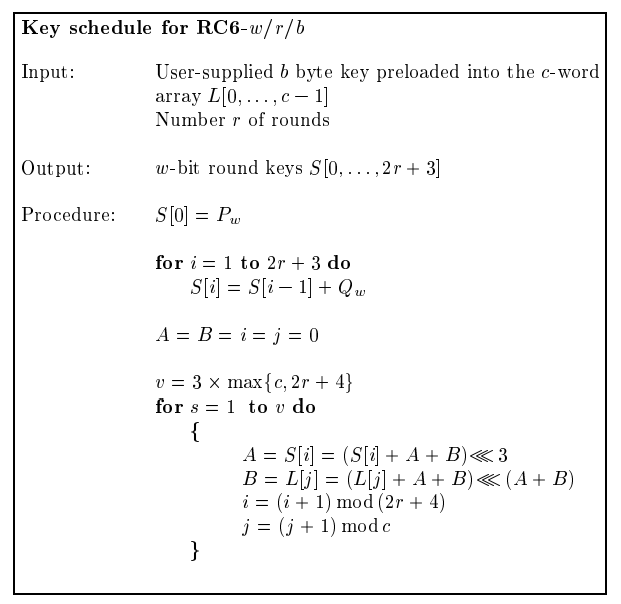
\includegraphics[width=0.5\linewidth]{rc_keys.png}
    \caption{Расписание ключей шифра RC6 [5]}
    \label{fig:enter-label}
\end{figure}

\textbf{Шифр RC6}

Этот алгоритм шифрования работает с 4 32-битными регистрами $(A, B, C, D)$, в которые загружается исходный 128-битный блок (в A загружается наименее значимый байт, в D - наиболее значимый байт). После работы алгоритма там будет находится шифротекст. Входом алгоритма являются количество раундов $r$ и вычисленные ключи раунда, находящиеся в $S$. Алгоритм выглядит следующим образом: 

\begin{figure}
    \centering
    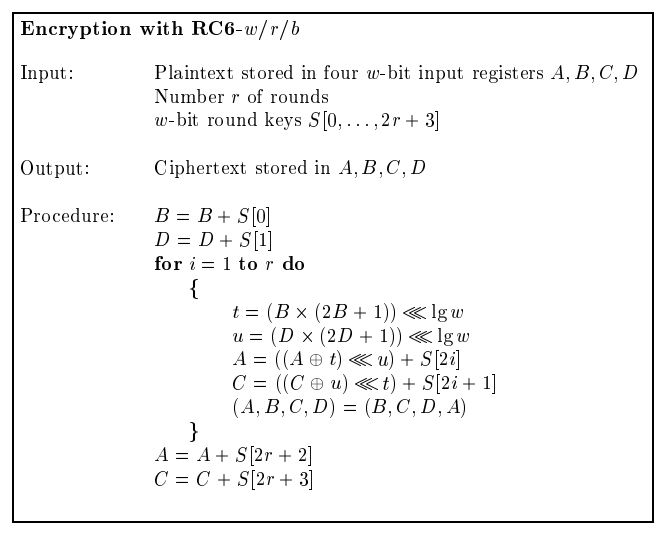
\includegraphics[width=0.5\linewidth]{rc6.png}
    \caption{Шифр RC6 [5]}
    \label{fig:enter-label}
\end{figure}

Переменная $w = 32$.

\subsubsection{Безопасность шифра}
На сегодняшний день не было опубликовано реальных атак на шифр RC6. Лучшей атакой на него является полный перебор секретного ключа.


\section{Список литературы}
[1] URL: https://academickids.com/encyclopedia/index.php/Image:DES-main-network.png (дата обращения: 13.01.2024)

[2] URL: https://academickids.com/encyclopedia/index.php/Image:DES-f-function.png (дата обращения: 13.01.2024)

[3] URL: https://academickids.com/encyclopedia/index.php/Image:DES-key-schedule.png (дата обращения: 13.01.2024)

[4] Daemen J., Rijmen V. AES proposal: Rijndael. – 1999.

[5] Rivest R. L. et al. The RC6TM block cipher //First advanced encryption standard (AES) conference. – 1998. – С. 16.

[6] URL: https://ru.wikipedia.org/wiki/ГОСТ\_28147-89#Достоинства\_стандарта (дата обращения: 16.01.2024)

[7] URL: https://ru.wikipedia.org/wiki/ГОСТ\_28147-89#/media/Файл:Feistel\_function\_GOST.png (дата обращения: 16.01.2024)

[8] Государственный стандарт СССР ГОСТ 28147-89. URL: https://files.stroyinf.ru/Data2/1/4294826/4294826631.pdf (дата обращения: 16.01.2024)

[9] URL: https://www.securitylab.ru/news/405678.php(дата обращения: 17.01.2024)

[10] URL: https://iacr.org/workshops/ches/ches2010/presentations/CHES2010\_Session05\_Talk02.pdf (дата обращения: 17.01.2024)
 
[11] URL: https://moluch.ru/archive/358/80031/ (дата обращения: 17.01.2024)

[12] Isobe T. A single-key attack on the full GOST block cipher //Journal of cryptology. – 2013. – Т. 26. – С. 172-189.

[13] Standard D. E. et al. Data encryption standard //Federal Information Processing Standards Publication. – 1999. – Т. 112.

[14] Biryukov A., Wagner D. Slide attacks //International Workshop on Fast Software Encryption. – Berlin, Heidelberg : Springer Berlin Heidelberg, 1999. – С. 245-259.

[15] Biryukov A., Wagner D. Advanced slide attacks //International conference on the theory and applications of cryptographic techniques. – Berlin, Heidelberg : Springer Berlin Heidelberg, 2000. – С. 589-606.

[16] Ростовцев А. Г. и др. О стойкости ГОСТ 28147-89 //Проблемы информационной безопасности. Компьютерные системы. – 2003. – №. 1. – С. 75-83.

[17] URL: https://files.stroyinf.ru/Data2/1/4293732/4293732907.pdf(дата обращения: 17.01.2024)

[18] Biryukov A., Perrin L., Udovenko A. Reverse-Engineering the S-Box of Streebog, Kuznyechik and STRIBOBr1 (Full Version) //Cryptology ePrint Archive. – 2016.

[19] AlTawy R., Youssef A. M. A meet in the middle attack on reduced round Kuznyechik //IEICE TRANSACTIONS on Fundamentals of Electronics, Communications and Computer Sciences. – 2015. – Т. 98. – №. 10. – С. 2194-2198.

[20] URL: https://en.wikipedia.org/wiki/International\_Data\_Encryption\_Algorithm(дата обращения: 17.01.2024)

[21] E. Biham, O. Dunkelman, N. Keller. A New Attack on 6-Round IDEA // Лекционные записи по теории вычислительных систем = Lecture Notes In Computer Science. — Berlin / Heidelberg: Springer-Verlag, 18 августа 2007 г. — P. 211—224.

[22] URL: https://web.archive.org/web/20070928014200/http://www.mediacrypt.com/\_pdf/NXT\_Technical\_Description\_0406.pdf (дата обращения: 17.01.2024)
\section{Приложение}

[23] Wu Z. et al. Impossible differential cryptanalysis of FOX //Cryptology ePrint Archive. – 2009.

\textbf{Блок Е шифра DES}


\begin{figure}[H]
    \centering
    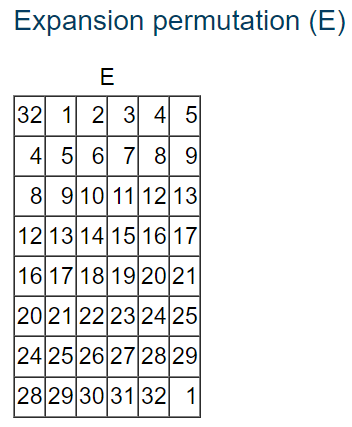
\includegraphics[width=0.25\linewidth]{e_perm.png}
    \label{fig:enter-label}
\end{figure}

\textbf{Блок P шифра DES}

\begin{figure}[H]
    \centering
    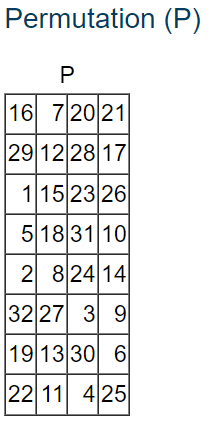
\includegraphics[width=0.25\linewidth]{perm.png}
    \label{fig:enter-label}
\end{figure}

\textbf{Блок PС1 шифра DES}

\begin{figure}[H]
    \centering
    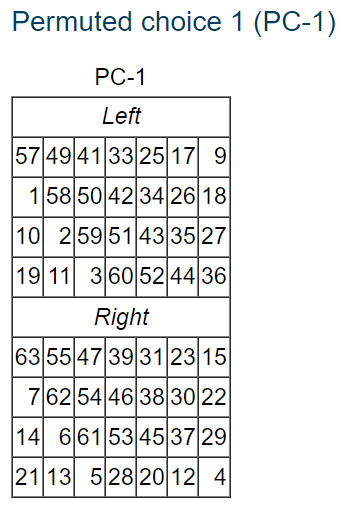
\includegraphics[width=0.25\linewidth]{pc1.png}
    \label{fig:enter-label}
\end{figure}

\textbf{Блок PС2 шифра DES}

\begin{figure}[H]
    \centering
    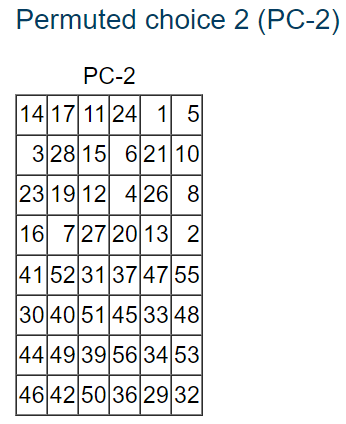
\includegraphics[width=0.25\linewidth]{pc2.png}
    \label{fig:enter-label}
\end{figure}

\textbf{Нелинейное преобразование шифра \textquotedblКузнечик\textquotedbl}

$Int_8$ - это представление 8-битовой последовательности как числа, $Vec_8$ - делает обратную операцию к $Int_8$.

\begin{figure}[H]
    \centering
    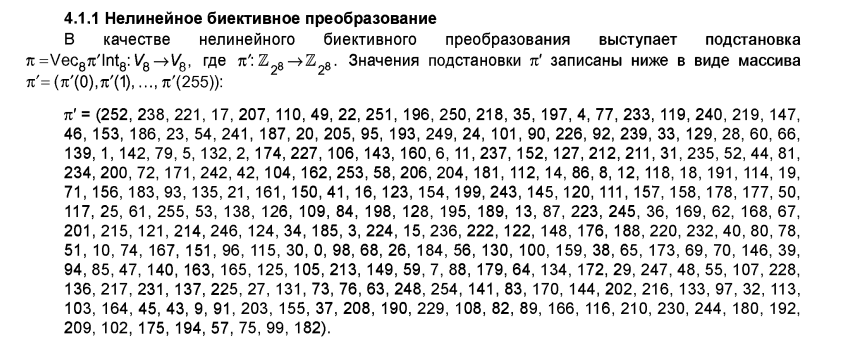
\includegraphics[width=0.5\linewidth]{permutation.png}
    \caption{Нелинейное преобразование шифра \textquotedblКузнечик\textquotedbl}
    \label{fig:enter-label}
\end{figure}

\end{document}
